\documentclass[11pt]{scrartcl}

\title{Analyse Bitnami}
\author{Silvan Adrian \\ Fabian Binna}
\date{\today{}}

\usepackage[ngerman]{babel}
\usepackage[automark]{scrpage2}
\usepackage[colorlinks = true,
linkcolor = black]{hyperref}
\usepackage{color}
\usepackage[normalem]{ulem}
\usepackage{scrpage2}
\usepackage{graphicx}
\usepackage{tabularx}
\graphicspath{ {../22_Grafiken/01_Logo/}{images/}{../../22_Grafiken/01_Logo/} }
\pagestyle{scrheadings}

\clearscrheadfoot
\ihead{
\includegraphics[scale=0.3]{SDDC}}
\ohead{Projekt: SDDC}
\ifoot{Template}
\cfoot{Version: 1.03}
\ofoot{Datum: \today{}}
\setheadsepline{0.5pt}
\setfootsepline{0.5pt}

\usepackage{ucs}
\usepackage[utf8]{inputenc}
\usepackage[T1]{fontenc}


\begin{document}
\def\arraystretch{1.5}
\begin{titlepage}
\begin{center}
\vspace{10em}

\includegraphics[scale=2]{SDDC}
\vspace{10em}
\end{center}
\begin{center}
\huge {Analyse Bitnami}
\end{center}
\begin{center}
\vspace{10em}
\LARGE {Silvan Adrian} \\
\LARGE {Fabian Binna}
\end{center}

\end{titlepage}

\newpage
\section{Änderungshistorie}
\begin{tabularx}{\linewidth}{l l X l}
\textbf{Datum} & \textbf{Version} & \textbf{Änderung}  & \textbf{Autor} \\
\hline
\textbf{25.09.15} & 1.00 & Erstellung des Dokuments & Gruppe \\
\textbf{25.09.15} & 1.01 & Einführung + Referenzen & Silvan Adrian \\
\textbf{25.09.15} & 1.02 & informationen zu Launchpads und Dashboard + 
Screenshots von den Möglichkeiten & Silvan Adrian \\
\textbf{25.09.15} & 1.03 & AWS \&Azure \& Google \& Digitalocean \& VMware & 
Silvan Adrian\\
\end{tabularx}

\newpage
\tableofcontents
\newpage

\section{Einführung}
\subsection{Zweck}
Dieses Dokument beinhaltet die Analyse vom Bitnami Dashboard.
\subsection{Gültigkeitsbereich}
Dieses Dokument ist während des ganzen Projekts gültig.

\subsection{Referenzen}
\textbf{Bitnami Consoles:}\\
\href{https://digitalocean.bitnami.com}{https://digitalocean.bitnami.com}\\
\href{https://azure.bitnami.com}{https://azure.bitnami.com}\\
\href{https://google.bitnami.com}{https://google.bitnami.com}\\
\href{https://vmware.bitnami.com/}{https://vmware.bitnami.com/}\\
\href{https://app.bitnamihosting.com/}{https://app.bitnamihosting.com/ (AWS)}\\

\section{Bitnami}
\subsection{Einführung}
Bitnami bietet ein Dashboard für einige Cloud Anbieter (VMware, AWS, Google Cloud, Azure, 
Digitalocean), um ganz einfach vorgegebene viel verwendete WebApps,Datenbanken oder Technologie Stacks 
schnell in der Cloud zu starten.
Dabei wird bei jedem eine Compute Instanz erstellt und das Image installiert.
Diese Analyse soll dabei helfen eine gute Lösung für unser Dashboard zu 
konzipieren und auf bereits bewährtes zurückgreifen können.

\subsection{Cloud Anbieter}
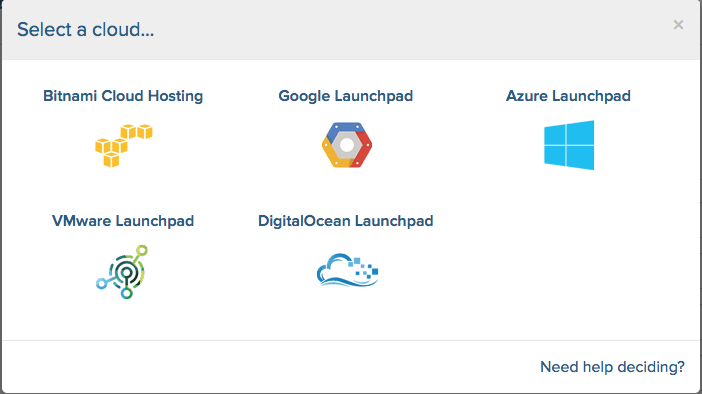
\includegraphics[width=\textwidth]{clouds}
\subsubsection{Bitnami Cloud Hosting}
Beim Bitnami Cloud Hosting steckt AWS dahinter, hier sind die meisten 
Einstellungen möglich im Vergleich zu den anderen Dashboards.


\textbf{Übersicht}
kurze Übersicht über die möglichen Konfigurationen einer AWS Instanz.
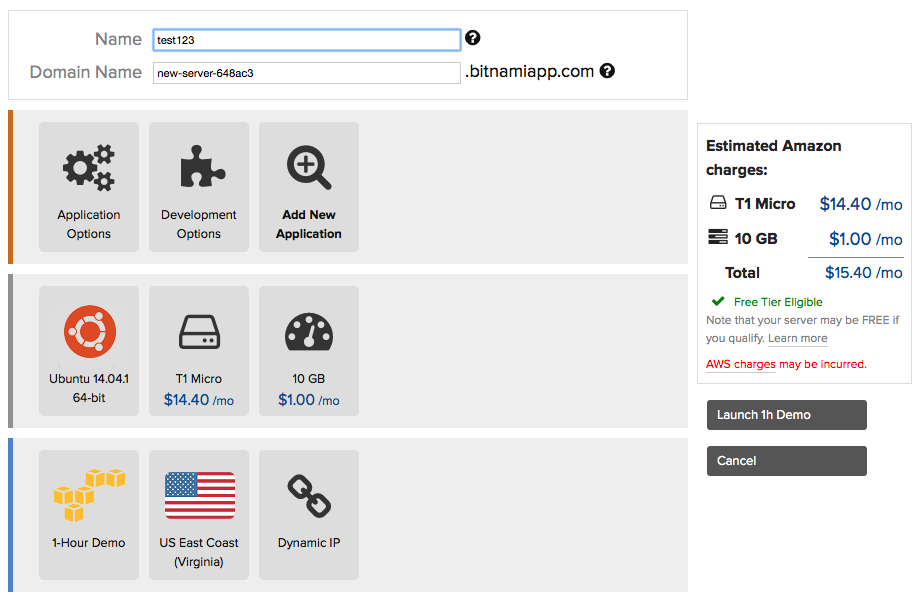
\includegraphics[width=0.8\textwidth]{aws_overview}
\newpage
\textbf{Application Options:}

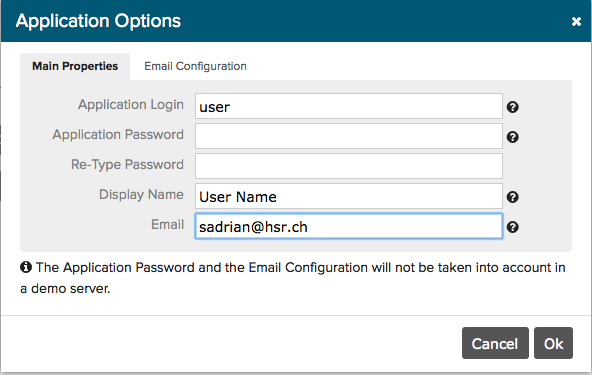
\includegraphics[width=0.5\textwidth]{aws_application_options}

\textbf{Applikationsauswahl:}

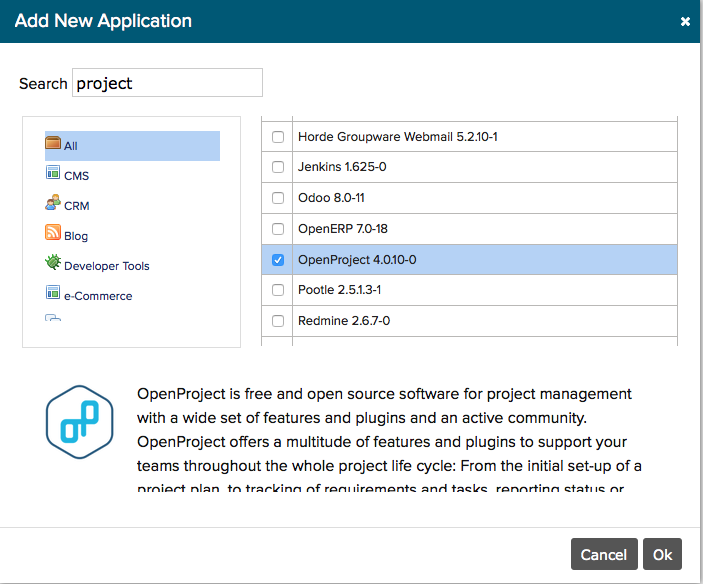
\includegraphics[width=0.5\textwidth]{aws_add_application}

\textbf{Betriebssystem:}

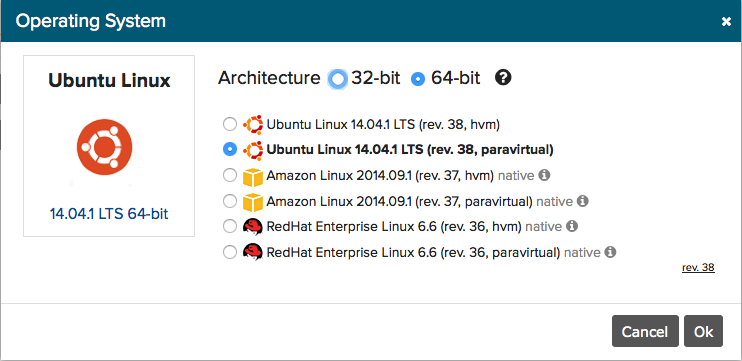
\includegraphics[width=0.5\textwidth]{aws_operating_system}

\textbf{Servertyp:}

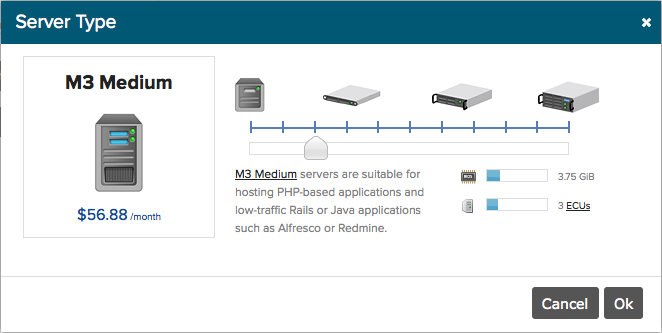
\includegraphics[width=0.5\textwidth]{aws_servertype}
\newpage
\textbf{Diskgrösse:}

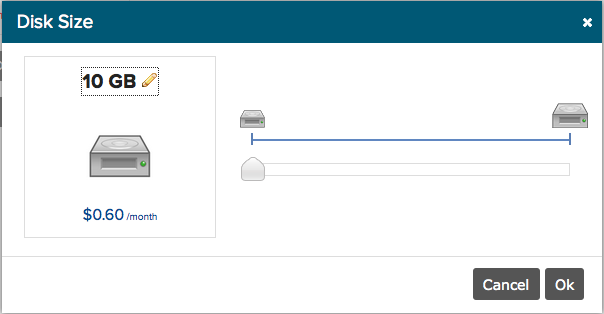
\includegraphics[width=0.5\textwidth]{aws_disk}

\textbf{Region,IP,Account:}

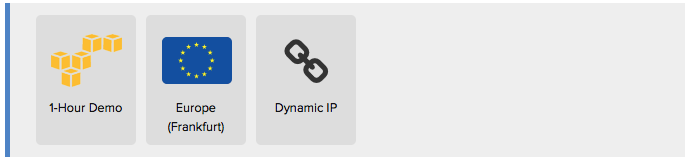
\includegraphics[width=0.5\textwidth]{aws_random}

\textbf{Management:}

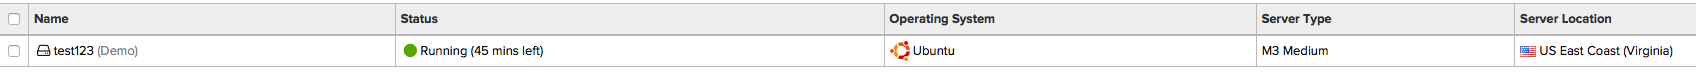
\includegraphics[width=\textwidth]{aws_overview_managment}

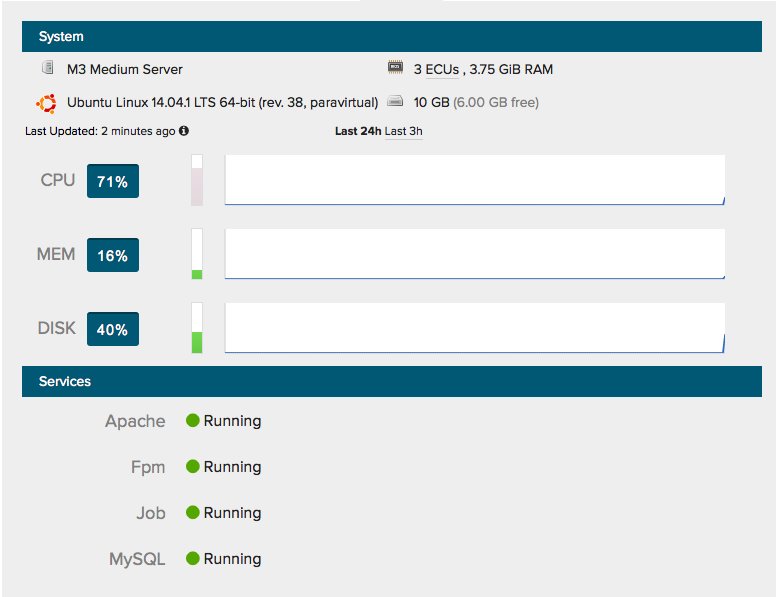
\includegraphics[width=0.5\textwidth]{aws_resourcen}

\textbf{Ressourcen:}

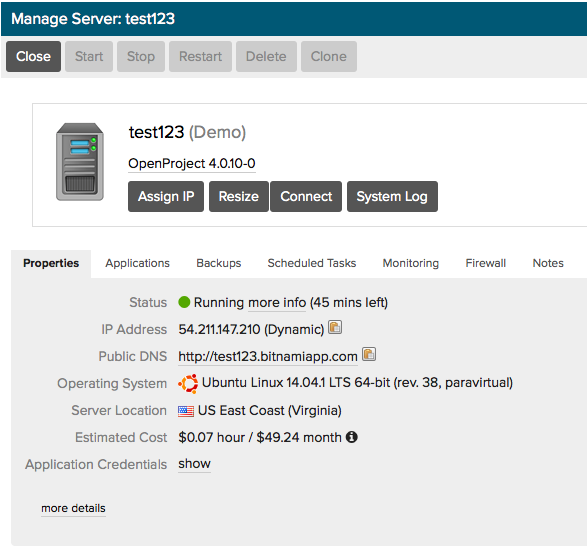
\includegraphics[width=0.5\textwidth]{aws_managment}

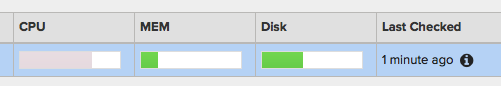
\includegraphics[width=0.5\textwidth]{aws_resrouces}

\newpage
\subsubsection{Digitalocean Launchpad}
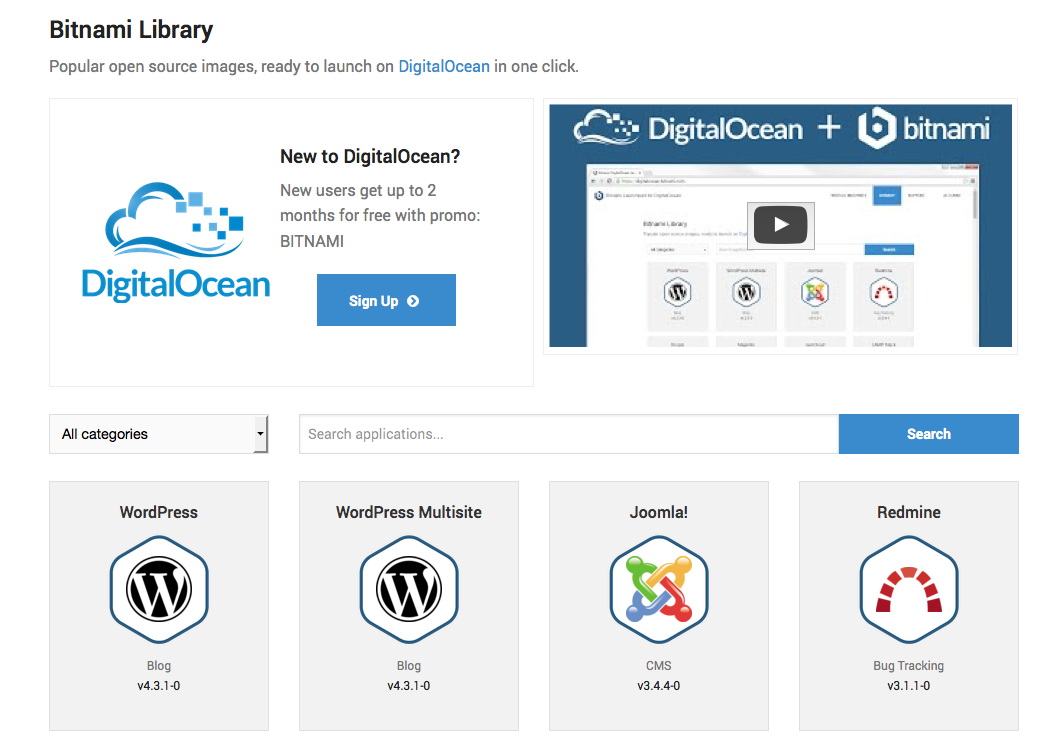
\includegraphics[width=\textwidth]{digitalocean_launchpad}
\textbf{Instanzen:}
Sobald eine Applikation ausgewählt wurde kann eine Instanz mit dem App gestartet 
werden, dabei kann noch die Instanzgrösse und Location gewählt werden.

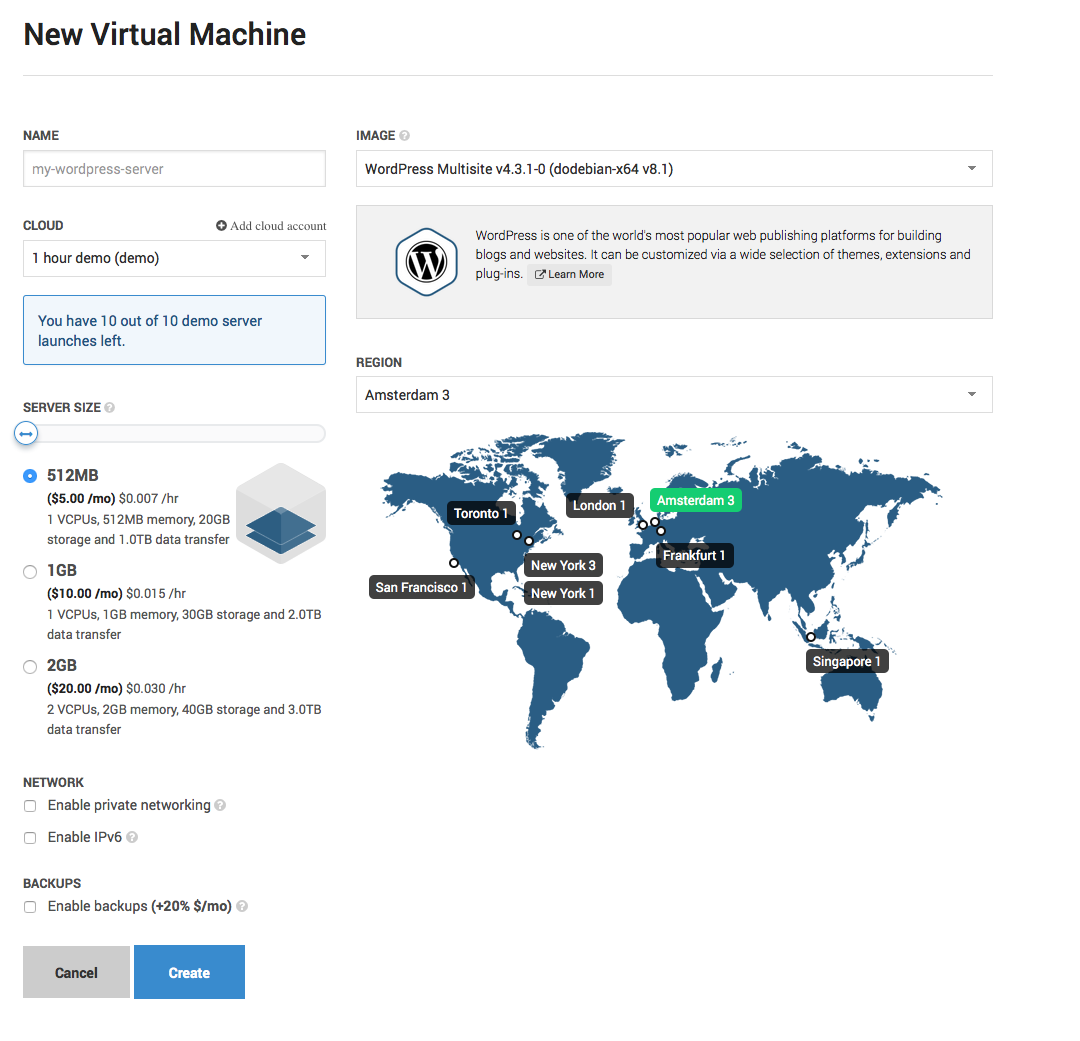
\includegraphics[width=\textwidth]{digitalocean_size}
Sobald Instanz erstellt lässt sich deren Status überprüfen + App spezifische 
Links werden gesetzt.

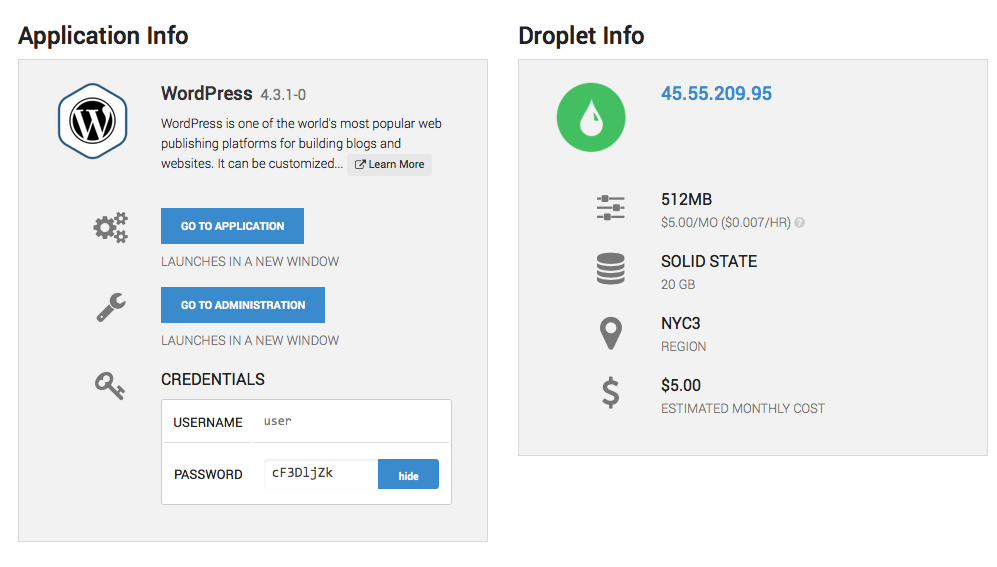
\includegraphics[width=\textwidth]{digitalocean_infos}

\textbf{Authorize Application:}
Um wirkliche Instanz erstellen zu können muss das Bitnami Dashboard Zugriff auf 
den Cloud spezifischen Account haben.

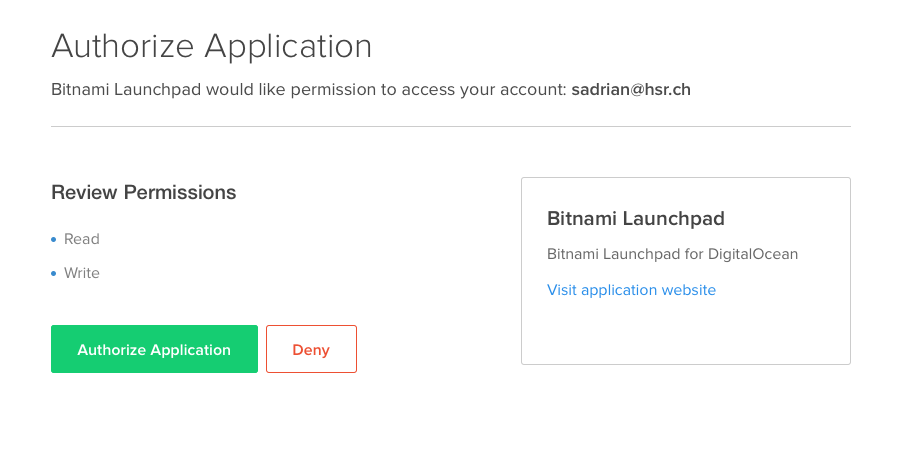
\includegraphics[width=\textwidth]{digitalocean_authorize}

Dabei können mehrere Accounts hinzugefügt werden:

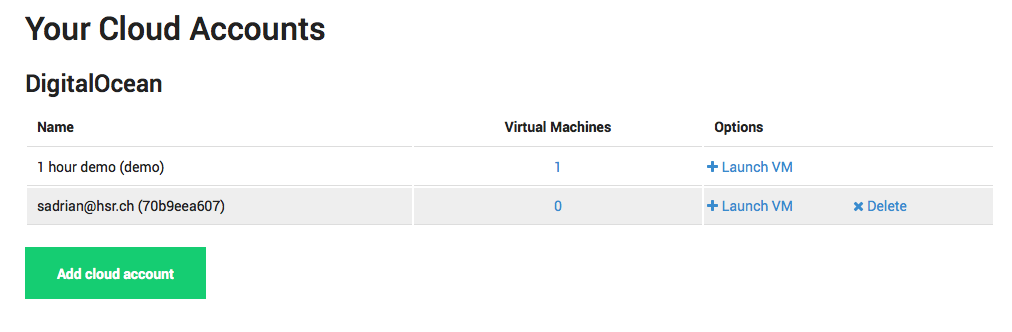
\includegraphics[width=\textwidth]{digitalocean_accounts}

Und unter jedem Account können spezifisch VM's erstellt werden:

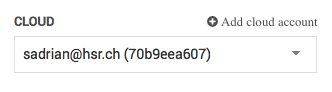
\includegraphics[width=0.4\textwidth]{digitalocean_account_specific}

Danach taucht die Instanz in der Übersicht auf:

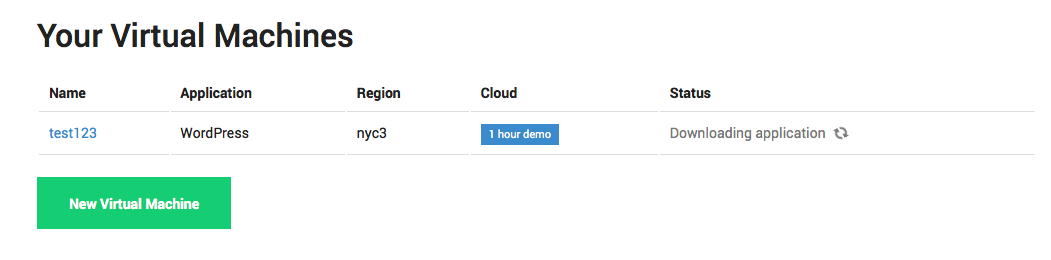
\includegraphics[width=\textwidth]{digitalocean_instances}

\newpage
\textbf{Instanzinfos:}

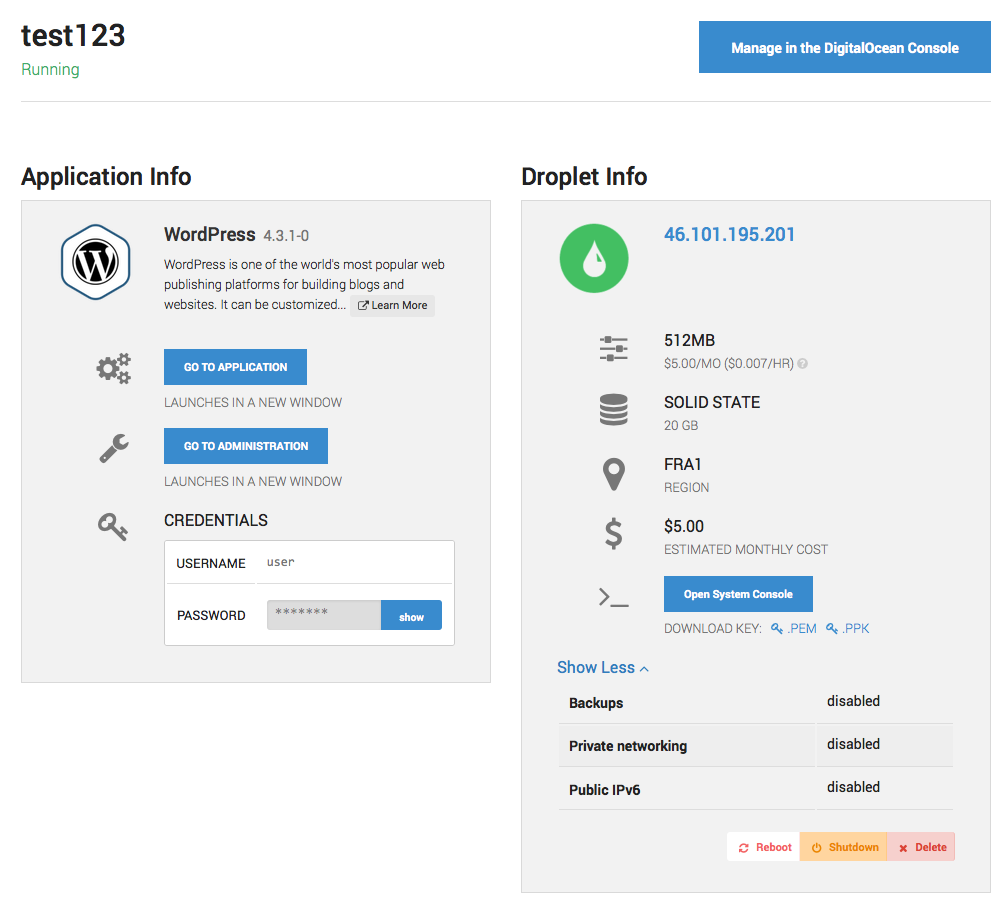
\includegraphics[width=\textwidth]{digitalocean_instanceinfo}

\subsubsection{Azure Launchpad}
Beim Azure Launchpad wird wieder gleich vorgegangen, wie bei Digitalocean.
Nur das sich die infos ändern (Bspw.: Bei Digitalocean Droplet, jetzt Server).

Ebenfalls ändern sich die Instanzgrössen. welche bei Azure anders als bei 
Digitalocean sind + wird bei Azure mit Subscriptions und nicht anhand von 
Accounts unterschieden.
\textbf{Serverinfo:}

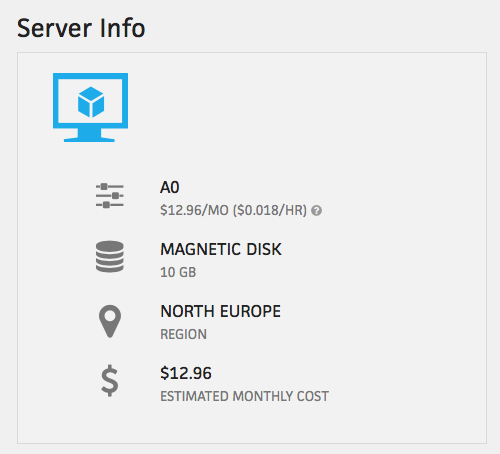
\includegraphics[width=0.5\textwidth]{azure_serverinfo}

\textbf{Authorization:}

Bei Azure wird das Dashboard über ein Managment Certificate autorisiert:

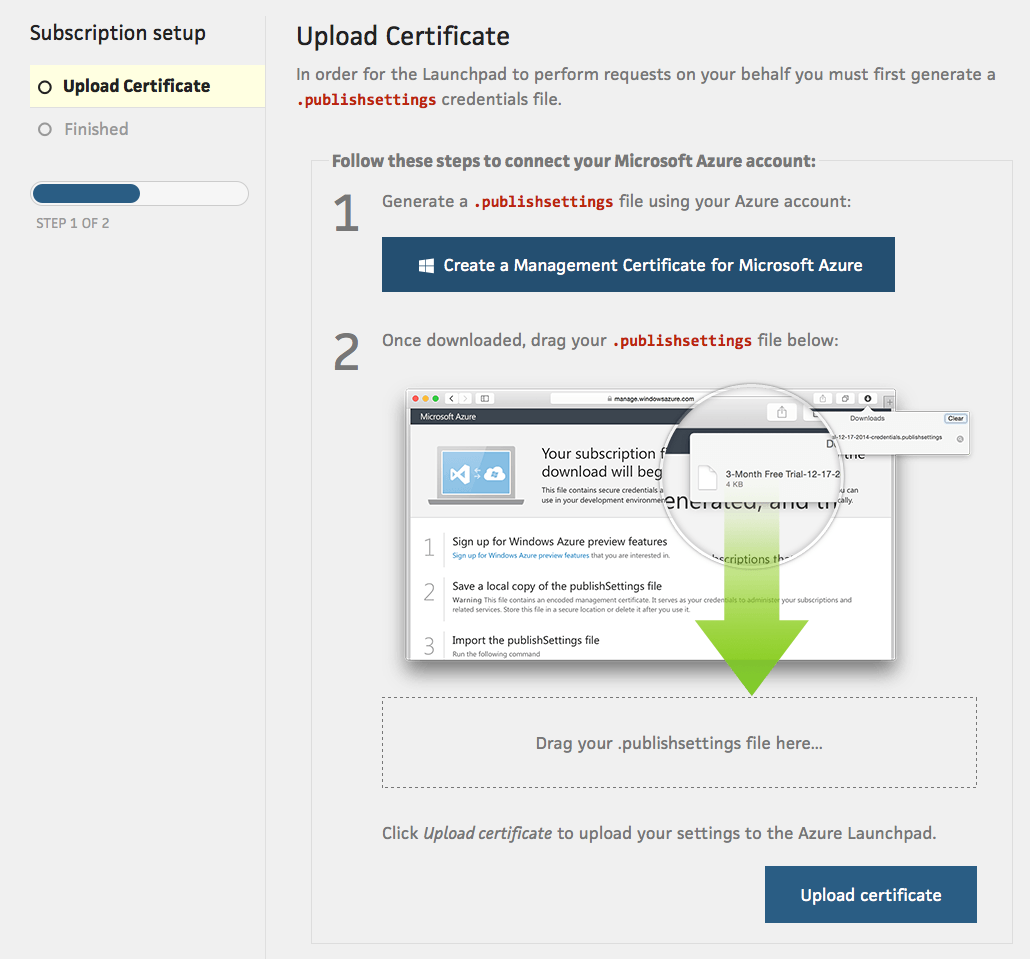
\includegraphics[width=0.8\textwidth]{azure_authorize}

Danach wird die vorhandene Subscription/s vom Microsoft Account eingebunden:

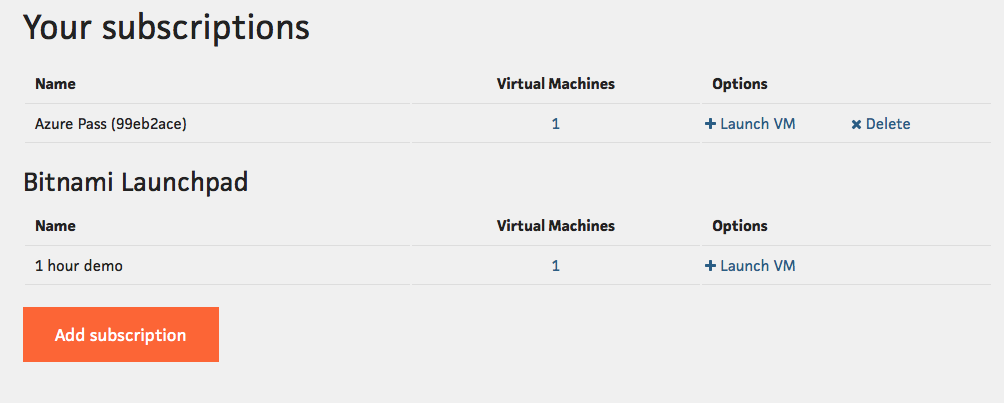
\includegraphics[width=0.8\textwidth]{azure_subscriptions}


Sobald dann ein neuer Server erstellt wurde kann dieser auch wieder gelöscht 
werden und all dessen Infos angesehen werden.

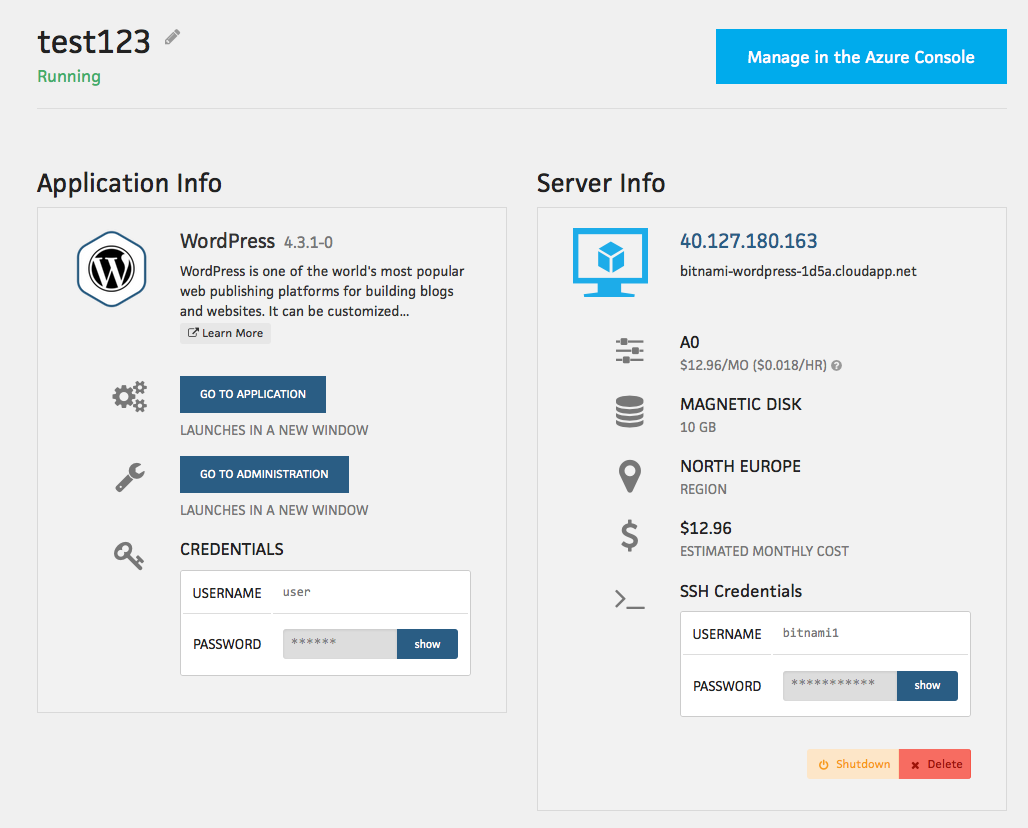
\includegraphics[width=0.8\textwidth]{azure_instanceinfos}

\subsubsection{Google Launchpad}

Beim Google Launchpad wieder dasselbe, wie bei Azure oder Digitalocean.
Hier wird einfach mit Projekten unterschieden (schliesslich kann jedem Projekt mehrere Compute Instanzen 
oder andere Services angefügt sein.)


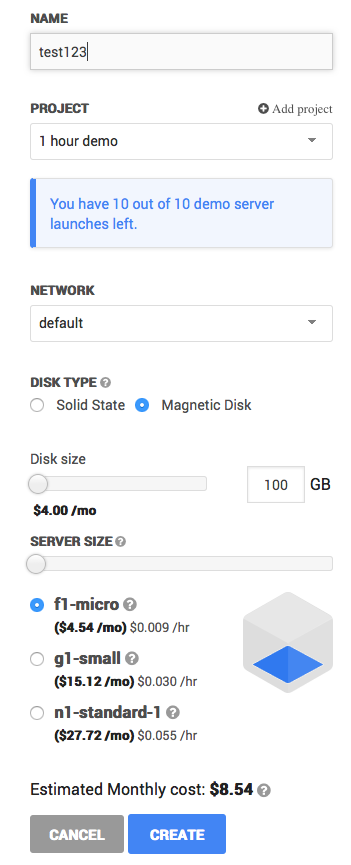
\includegraphics[width=0.4\textwidth]{google_instancereation}


\subsubsection{VMware Launchpad}
Das VMware Launchpad kann für die WMware vCloud Air gebraucht werden.

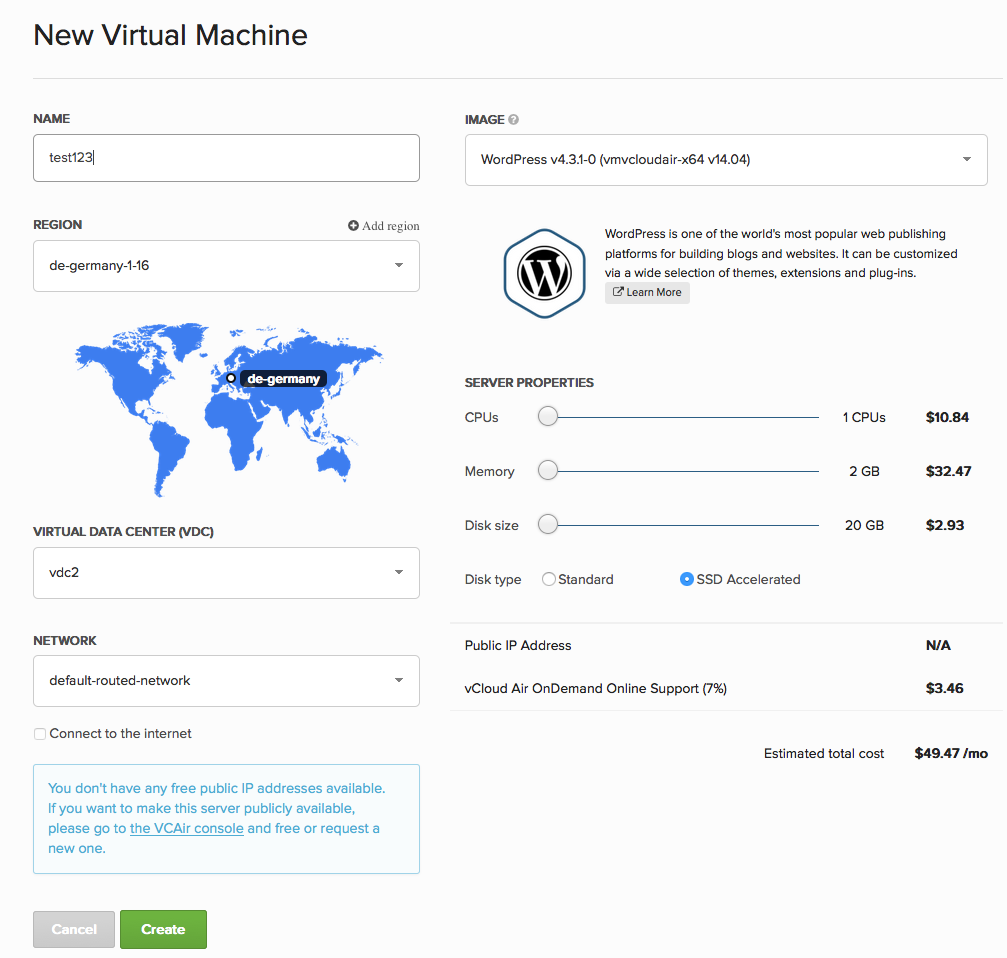
\includegraphics[width=0.8\textwidth]{vmware_creation}

\textbf{Infos:}

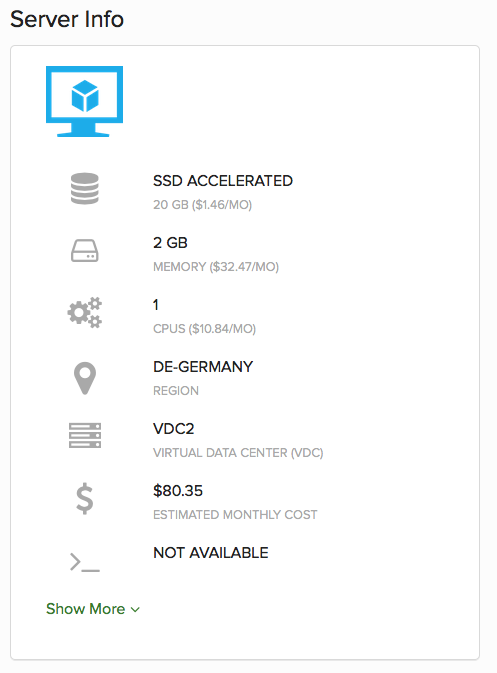
\includegraphics[width=0.4\textwidth]{vmware_infos}

\subsection{Security}
Da durch das zentrale zusammenfassen von mehreren Accounts auch immer 
Sicherheitsrisiken zu beachten sind, wird bei Bitnami zusätzlich zum normalen 
Loginpasswort auch noch ein Vaultpasswort festgelegt, welches wohl die 
Logindaten symmetrisch verschlüsselt und in einem ``Vault'' ablegt.

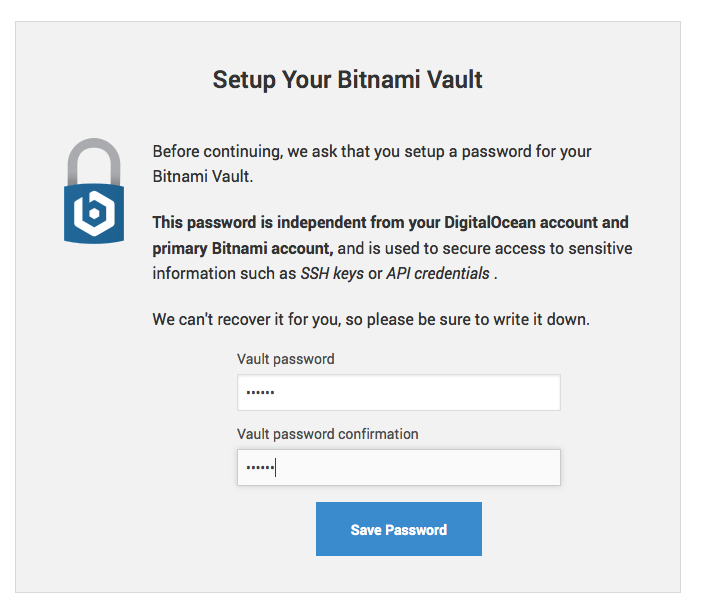
\includegraphics[width=0.8\textwidth]{bitnami_security}

\subsection{Applikationen}
Die Applikationen können sich von Anbieter zu Anbieter unterscheiden, jedoch 
gibt es für sehr viel verwendete Applikationen (Bspw.: Wordpress) bei jedem ein 
Image.
Es besteht bereits eine sehr grosse Auswahl für sehr viel verschiedene Apps und 
es werden immer mehr, wodurch es immer einfacher wird schnell eine Applikation 
aufzusetzen.
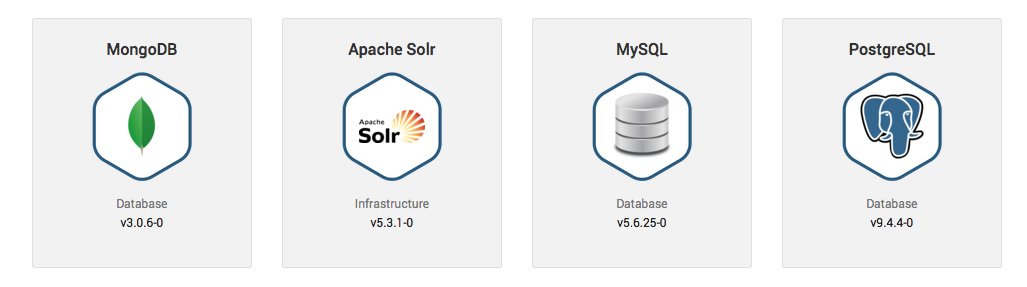
\includegraphics[width=\textwidth]{apps}

\subsubsection{Kategorien}
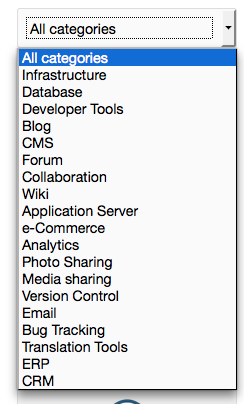
\includegraphics[width=0.3\textwidth]{categories}

\section{Fazit}
Bitnami bietet einiges was Computing angeht und ist der einzig grössere 
Dashboard Anbieter, der mehrere verschiedene Cloud Anbieter unterstützt.
Allerdings fehlen verschiedene PaaS Angebote (Bspw.: Cloud SQL bei Google etc.), 
Bitnami ist daher nur für eigene Instanzen/Vms zu gebrauchen und nicht mit einer 
generellen Service Unterstützung konzipiert worden.
Das Dashboard bei Bitnami bietet jedenfalls einiges und gibt einem einen guten 
Überblick über seine eigenen abonnierten Services (VM Instanzen).


\end{document}